\section{The {\tt FOR} language}
\label{sec:FOR}
\begin{table}[htb]
	\begin{grammar}
		<expression> ::= 
							`nil' 
				\alt 	`cons' <expression> <expression>
				\alt 	`hd' <expression>
				\alt 	`tl' <expression>
				\alt 	<variable>

		<statement-list> ::= <statement> ;\alt <statement> ; <statement-list>

		<block> ::= `{' <statement-list> `}'

		<statement> ::=
							<variable> `:=' <expression>
				\alt	`if' <expression> <block> <else-block>
				\alt	`for' <variable> `in' <expression> <block>
			
				<else-block> ::= <empty> \alt `else' <block>
				
				<program> ::= <name> `read' <variable> <block> `write' <variable>
	\end{grammar}
	\caption{The \FOR syntax \label{tab:FOR-syntax}}
\end{table}

\subsection{The Elements} % (fold)
\label{sub:The Elements}
The \FOR language contains only very basic commands, but they can be combined
to implement a huge number of algorithms. As the data structure, we choose 
the humble {\tt cons} cell, that contains only a reference as the head and 
another as the tail.\footnote{An observant reader will notice that this
structure stems from the building of linked lists.}
.
\begin{figure}[htb]
	\begin{center}
		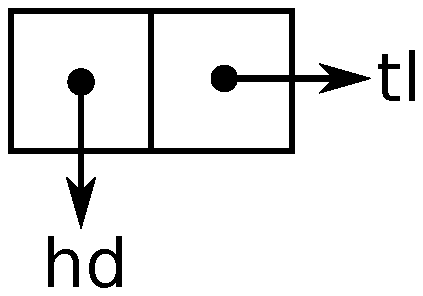
\includegraphics[height=3cm]{introduction/for/images/conscell}
	\end{center}
	\caption{The {\tt cons} cell}
\end{figure}

The expression {\tt cons e1 e2} constructs such a cell with the evaluation of
e1 in the head and the evaluation of e2 in the tail. The expression {\tt hd e1}
yields the head of the evaluation of e1 and {\tt tl e1} its tail. Since all our
current constructs need another expression, we also need a "bottom" to this
regress. We add {\tt nil} as an expression, which is distinct from any {\tt
cons e f}. We also want to refer to stored values, so an identifier (eg {\tt
X}) can also be an expression.

There are very few types of statements in \FOR, just three to be precise. The 
first is the {\em assignment} {\tt X := e}, which assigns the variable {\tt X}
the evaluation of {\tt e}. Later, when {\tt X} is used in an expression, it 
will reproduce this value. The second is the classic {\tt if} statement, that 
only executes its first block, if the expression does {\em not} return {\tt nil} 
and the else-block -- if any -- otherwise. Finally, there is the eponymous 
{\tt for} loop, that works as follows:

\begin{enumerate}
	\item On first entering the loop, the expression is evaluated and lets call 
		it $e$.
	\item If the evaluation is {\tt nil}, the loop is not evaluated anymore.
	\item Otherwise the block is evaluated with the value of the head of $e$.
	\item Then this procedure is run again with the tail of $e$.
\end{enumerate}

\subsection{\FOR computability}
The probably most important property of the \FOR language is that programs in 
it always terminate. The reason for this is, that upon entering the for loop, 
the number of repetitions is fixed as the length of the evaluated expression. 
Since we can't build an infinite expression in the finite time before the 
loop, the program terminates.

When experimenting with the language, one quickly finds, that many important 
functions are \FOR computable:

\begin{itemize}
	\item Constant functions.
	\item Addition.
	\item Multiplication -- as repeated addition.
	\item Exponentiation -- as repeated multiplication.
	\item Unary/binary conversion.
	\item Testing if a given number is prime.
	\item ...
\end{itemize}

As we can see, it is relatively simple to generate huge numbers using the 
\FOR language and then generate lists with that length.

\lineofthought{Thm: Algorithm $C$ with $T(C)\in O(f(n))$, $f(n) \in \FOR$, 
	then $\interpret{C}\in \FOR$}

At first glance it seems that any function can be computed this way, but 
sadly, that is not the case.

Intuitively the interpretation of a \FOR program should be computable. We can 
do it in an algorithmic way and so it is only reasonable to expect \FOR to be 
able to interpret itself. As we will see, that can not be the case:

\begin{theorem}
	There is no \FOR program $exec$ that takes $(program.input)$ as its 
	argument and returns $\interpret{program}(input)$.
\end{theorem}
\begin{proof}
Assume, there was a procedure in \FOR $exec$ that takes $(program.input)$ as 
its argument. Now the following procedure would surely be a \FOR program too:

\begin{verbatim}
inverse read X {
  result := [exec](X.X)
  if result {
    Y := FALSE
  } else {
    Y := TRUE
  }
} write Y
\end{verbatim}

We have 
\[ \interpret{inverse}(program) = \begin{cases}
		\mathtt{TRUE}, &\text{ if }\interpret{program}(program) = \mathtt{FALSE} \\
		\mathtt{FALSE}, &\text{ otherwise }
	\end{cases} \]

It outputs {\tt TRUE} iff the given program outputs {\tt FALSE}. What then 
is $\interpret{inverse}(inverse)$? Assume first that it is 
{\tt TRUE}, then by definition it is {\tt FALSE} -- and vice versa! So it 
neither returns {\tt TRUE} {\em nor} {\tt FALSE}. The only way that would 
work would be if it didn't return anything at all, but as we have seen, all 
\FOR programs terminate in finite time, so that can not be the case. 
Therefore {\tt inverse} can not be a \FOR program and by extension {\tt exec} 
is not a \FOR program. 
\footnote{This is the quitessential uncomputability 
	proof: A coding of the function is given that can be evaluated, but running 
  the program on itself leads to complications.}
\end{proof}

This is unfortunate, not only because we have seen that there are functions 
that are not \FOR computable, but that in general, any language that supports 
the building blocks of {\tt inverse} either doesn't support 
self-interpretation or it contains programs that will not halt.

As we try to capture {\em all} intuitively computable functions, it is not 
acceptable to leave self-interpretation out, so in the next chapter, we will 
explore a language that will contain non-halting programs.

\subsection{The \FOR in real programming languages}
It turns out, that while the {\tt for} keyword exists in most languages in 
one form or another, few acurately model the \FOR languages intention. 
Foremost most languages cheat around the property of \FOR loops always 
terminating: In C-like languages, the loop variable is not immutable and therefore
\begin{verbatim}
	for (int i = 0; i < 10; i++) {
	  // ...
	}
\end{verbatim}
might very well not terminate, if {\tt i} is decremented in the body. 
Iterator-based loops can be tricked by implementing an iterator that does not 
halt, i.e. produces a new value on any {\tt next}.

\subsection{The \FOR in mathematics and logic}
The \FOR computable functions match a category of functions known as 
primitive recursive. A function is primitive recursive, if it is either
\begin{enumerate}
	\item A successor function $S_i(x_1,\dots,x_n) = x_i+1$
	\item A projection function $P_i(x_1,\dots,x_n) = x_i$
	\item In the form of primitive recursion:
		\begin{equation*}
			f(n,x_1,\dots,x_n) = \begin{cases}
				g(x_1,\dots,x_n), &\text{ if }n=0\\
				h(f(n-1, x_1, \dots, x_n), x_1,\dots,x_n),&\text{ else}
			\end{cases}
		\end{equation*}
		Where $g$ and $h$ are primitive recursive.
\end{enumerate}
It is easy to see that \FOR can compute any primitive recursive function:
The successor function and the projections are trivial, for the primitive 
recursion, we have programs $\interpret{G}=g$ and $\interpret{H}=h$ by 
induction assumtion\citationneeded. 

\begin{verbatim}
F read NX {
  N := hd NX
  Xs := tl NX
  Repetitions := [unary](N)
  Result := [G](Xs)
  Counter := 0
  FOR I IN Repetitions {
    Result := [H](Result.Xs)
  }
} write Result
\end{verbatim}

The other direction is in the exercises \TODO.
